\documentclass[11pt]{article}
\usepackage[a4paper,margin=2.2cm]{geometry}
\usepackage[T1]{fontenc}
\usepackage{lmodern}
\usepackage{amsmath,amssymb}
\usepackage{xcolor}
\usepackage{graphicx}
\usepackage{titlesec}
\usepackage{enumitem}
\usepackage[most]{tcolorbox}

\definecolor{hd}{RGB}{20,60,130}
\definecolor{kw}{RGB}{120,60,0}
\titleformat{\section}{\color{hd}\Large\bfseries}{}{0pt}{}
\titleformat{\subsection}{\color{hd}\bfseries}{}{0pt}{}
\titlespacing*{\subsection}{0pt}{10pt}{4pt}
\setlength{\parindent}{0pt}
\setlength{\parskip}{5pt}
\setlist{nosep,itemsep=2pt}

\newcommand{\pd}{\partial}
\newcommand{\bu}{\mathbf u}
\newcommand{\bo}{\boldsymbol\omega}
\newcommand{\kw}[1]{{\color{kw}\itshape ``#1''}}
\newtcolorbox{strategy}{colback=hd!5,colframe=hd!60,boxrule=0.5pt,arc=2pt,left=5pt,right=5pt,top=3pt,bottom=3pt,fonttitle=\bfseries\small,title=Strategy}
\newcommand{\why}[1]{{\color{gray}\small[#1]}}

\begin{document}
\begin{center}
{\color{hd}\Large\bfseries Physics of Fluids (PHYSFLU) --- Midterm Exam 2025--2026}\\[3pt]
Detailed resolution
\end{center}

%==================================================================
\section*{Problem 1 \normalsize(1.0 p.)}

\begin{strategy}
A stream function exists iff the 2D flow is incompressible ($\nabla\!\cdot\bu=0$). A potential exists iff it is irrotational ($\bo=0$). So: check the condition first, then construct the function by integrating one component and fixing the integration ``constant'' (a function of the other variable) with the other component.
\end{strategy}

\subsection*{(a) Incompressible? Stream function}
\[
\nabla\!\cdot\bu=\frac{\pd u}{\pd x}+\frac{\pd v}{\pd y}=2ax-2ax=0 .
\]
Yes, it can represent an incompressible flow. Construct $\Psi$ with $u=\pd_y\Psi$, $v=-\pd_x\Psi$:
\begin{enumerate}[label=\arabic*.]
\item Integrate $u$ in $y$: $\Psi=\int a(x^2-y^2)\,dy=a\left(x^2y-\frac{y^3}{3}\right)+f(x)$. The ``constant'' may depend on $x$.
\item Impose $v=-\pd_x\Psi$: $-2axy-f'(x)=-2axy\ \Rightarrow\ f'(x)=0$, so $f$ is an irrelevant constant.
\end{enumerate}
\[
\boxed{\Psi=a\left(x^2y-\frac{y^3}{3}\right)}
\]

\subsection*{(b) Irrotational? Potential}
\[
\omega_z=\frac{\pd v}{\pd x}-\frac{\pd u}{\pd y}=-2ay-(-2ay)=0 .
\]
Yes, it can represent an irrotational flow. Construct $\Phi$ with $u=\pd_x\Phi$, $v=\pd_y\Phi$:
\begin{enumerate}[label=\arabic*.]
\item $\Phi=\int a(x^2-y^2)\,dx=a\left(\frac{x^3}{3}-xy^2\right)+g(y)$.
\item $\pd_y\Phi=-2axy+g'(y)=v=-2axy\ \Rightarrow\ g'=0$.
\end{enumerate}
\[
\boxed{\Phi=a\left(\frac{x^3}{3}-xy^2\right)}
\]
Checks: $\nabla^2\Phi=2ax-2ax=0$ and $\nabla^2\Psi=2ay-2ay=0$, as required for an incompressible and irrotational flow. Both are parts of the complex potential $F=\Phi+i\Psi=\frac a3z^3$; this is the flow in a $60^\circ$ corner.

%==================================================================
\section*{Problem 2 \normalsize(3.0 p.)}

\begin{strategy}
Keywords: \kw{very long belt}, \kw{steady}, $\bu=(u(y),0,0)$ $\Rightarrow$ parallel flow on an inclined plane (a gravity film), with the wall \emph{moving}.
BCs: \kw{oil sticks to the belt} $\to$ no slip, $u(0)=$ belt velocity; \kw{external pressure $p_0$} acting on the free surface $\to$ $p(h)=p_0$ and zero shear stress, $u'(h)=0$.
Gravity has a component along the belt (drives the oil down) and one normal to it (hydrostatic pressure).
\end{strategy}

\textbf{Axes and signs (figure b).} $x$ runs along the belt pointing \emph{down} the slope, and $y$ is normal to the belt, pointing out of it. The belt moves up the slope, so the oil at $y=0$ has velocity $u(0)=-U$. Gravity components:
\[
g_x=+g\sin\theta,\qquad g_y=-g\cos\theta .
\]

\subsection*{(a) Velocity and pressure}
\textbf{Continuity.} $\pd_xu=0$ is satisfied by $u=u(y)$. The convective term $(\bu\cdot\nabla)\bu=u\,\pd_xu\,\hat x=0$: the flow is exactly parallel, so NS becomes linear.

\textbf{$y$-momentum (pressure).} $0=-\pd_yp+\rho g_y=-\pd_yp-\rho g\cos\theta$. Integrating with $p(h)=p_0$ at the free surface:
\[
\boxed{p(y)=p_0+\rho g\cos\theta\,(h-y)}
\]
This is hydrostatic pressure, with only the component of $g$ normal to the belt. It does not depend on $x$, so $\pd_xp=0$: the oil is driven only by gravity and the belt.

\textbf{$x$-momentum (velocity).}
\[
0=-\underbrace{\pd_xp}_{0}+\rho g\sin\theta+\mu u''\ \Rightarrow\ u''=-\frac{g\sin\theta}{\nu}
\ \Rightarrow\ u=-\frac{g\sin\theta}{2\nu}y^2+C_1y+C_2 .
\]
BCs: free surface $u'(h)=0\Rightarrow C_1=\frac{g\sin\theta}{\nu}h$; no slip on the belt $u(0)=-U\Rightarrow C_2=-U$.
\[
\boxed{u(y)=-U+\frac{g\sin\theta}{\nu}\left(hy-\frac{y^2}{2}\right)}
\]
The velocity is a uniform upward motion $-U$ (dragged by the belt) plus the half-parabola of a film falling freely under gravity. Since $u'=\frac{g\sin\theta}{\nu}(h-y)\ge0$, $u$ grows monotonically from $-U$ at the belt to its maximum at the surface:
\[
u(h)=-U+\frac{gh^2\sin\theta}{2\nu}.
\]

\subsection*{(b) Points at rest, and the minimum $U$}
A point is at rest where $u(y^*)=0$, with $0\le y^*\le h$. Because $u$ is monotonic, increasing from $u(0)=-U<0$, a zero exists inside the layer iff $u(h)\ge0$:
\[
U\le U_{\min}\equiv\frac{gh^2\sin\theta}{2\nu}.
\]
Its position solves $\frac{g\sin\theta}{\nu}\left(hy-\frac{y^2}{2}\right)=U$, i.e.\ $y^2-2hy+\frac{2\nu U}{g\sin\theta}=0$. Taking the root inside $[0,h]$:
\[
\boxed{y^*=h-\sqrt{h^2-\frac{2\nu U}{g\sin\theta}}}\qquad(U\le U_{\min}).
\]
\begin{itemize}
\item $U<U_{\min}$: the oil below $y^*$ goes up with the belt, and the oil above $y^*$ slides down.
\item $U=U_{\min}$: $y^*=h$, the surface is at rest.
\item $U>U_{\min}$: $u<0$ everywhere, so the whole layer moves upwards.
\end{itemize}
So yes: the whole layer moves upwards iff $\boxed{U>U_{\min}=\dfrac{gh^2\sin\theta}{2\nu}}$.

\begin{center}
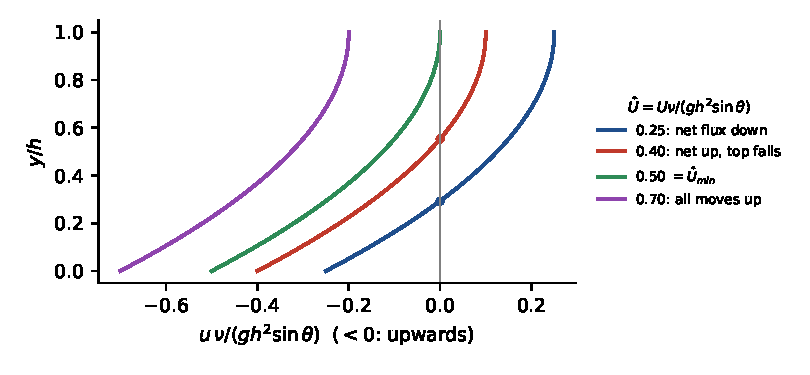
\includegraphics[width=0.78\textwidth]{t25_p2.pdf}
\end{center}

\subsection*{(c) Volumetric flux}
Per unit width of the belt (positive = down the slope):
\[
q=\int_0^hu\,dy=-Uh+\frac{g\sin\theta}{\nu}\left(\frac{h^3}{2}-\frac{h^3}{6}\right)
\ \Rightarrow\
\boxed{q=-Uh+\frac{gh^3\sin\theta}{3\nu}}
\]
The device lifts oil to the upper tank iff the net flux is upwards, $q<0$:
\[
\boxed{U>\frac{gh^2\sin\theta}{3\nu}}
\]
\textbf{Comment.} This threshold is \emph{lower} than $U_{\min}$ from (b), by a factor $2/3$. For $\frac{gh^2\sin\theta}{3\nu}<U<\frac{gh^2\sin\theta}{2\nu}$, the top of the layer still slides down, but the oil carried up near the belt outweighs it, so the device still works (red curve in the figure).

%==================================================================
\section*{Problem 3 \normalsize(2.0 p.)}

\begin{strategy}
Potential flows superpose: $\Psi=\sum\Psi_i$ because Laplace's equation is linear. Velocities: $u_r=\frac1r\pd_\theta\Psi$, $u_\theta=-\pd_r\Psi$. Stagnation points: both components zero. For (c), the complex velocity $\frac{dF}{dz}=u-iv$ makes the algebra short, since every vortex contributes a simple term.
\end{strategy}

\subsection*{(a) Stream function, velocity, circulation}
\[
\Psi=U_\infty r\sin\theta-A\ln r .
\]
\[
u_r=\frac1r\frac{\pd\Psi}{\pd\theta}=U_\infty\cos\theta,\qquad
u_\theta=-\frac{\pd\Psi}{\pd r}=-U_\infty\sin\theta+\frac{A}{r}.
\]
\why{The vortex part $u_\theta=A/r>0$ is anticlockwise, as stated.}
On a circle of radius $r$, $d\mathbf l=r\,d\theta\,\hat\theta$:
\[
\Gamma=\oint u_\theta\,r\,d\theta=\int_0^{2\pi}\left(-U_\infty r\sin\theta+A\right)d\theta=\boxed{2\pi A}
\]
The uniform stream contributes nothing (it is irrotational and has no singularity). Only the vortex contributes, the same for every $r$.

\subsection*{(b) Non-dimensionalisation and stagnation point}
With $\Gamma=2\pi A$, the scales are $\vec u'=\vec u/U_\infty$ and $r'=r\,\frac{2\pi U_\infty}{\Gamma}=\frac{rU_\infty}{A}$, i.e.\ lengths in units of $A/U_\infty$. Dividing the velocity by $U_\infty$:
\[
u_r'=\cos\theta,\qquad u_\theta'=-\sin\theta+\frac{1}{r'} .
\]
The problem now has no parameters. Stagnation point:
\begin{itemize}
\item $u_r'=0\Rightarrow\cos\theta=0\Rightarrow\theta=\pm\pi/2$.
\item $u_\theta'=0\Rightarrow\sin\theta=1/r'>0\Rightarrow\theta=+\pi/2$ (the minus sign would need $r'<0$), and then $r'=1$.
\end{itemize}
\[
\boxed{P_1:\ (r',\theta)=(1,\pi/2),\ \text{i.e. }(x',y')=(0,1)}\qquad\left(\text{dimensional: }y=A/U_\infty\right).
\]
\why{Physically: above the vortex, its anticlockwise velocity points in $-x$, against the stream. At distance $A/U_\infty$ the two cancel.}

\subsection*{(c) Adding two vortices to create $P_2=(0,-1)$}
\textbf{Complex velocity.} In dimensionless form ($U_\infty=A=1$), a uniform stream is $F=z$ and an anticlockwise vortex at $c$ is $F=-i\ln(z-c)$ (since $\operatorname{Im}[-i\ln z]=-\ln r$). With two new vortices at $c_1$, $c_2$:
\[
\frac{dF}{dz}=u'-iv'=1-\frac{i}{z}-\frac{i}{z-c_1}-\frac{i}{z-c_2}.
\]
\textbf{Condition 1: keep $P_1=i$ a stagnation point.} The first two terms already cancel at $z=i$ ($1-i/i=0$), so the new pair must give zero velocity there:
\[
\frac{1}{i-c_1}+\frac{1}{i-c_2}=0\ \Rightarrow\ i-c_1=-(i-c_2)\ \Rightarrow\ \frac{c_1+c_2}{2}=i .
\]
The two vortices must be placed symmetrically about $P_1$: $c_{1,2}=i\pm w$. \why{Two equal vortices induce opposite velocities only at their midpoint.}

\textbf{Condition 2: make $P_2=-i$ a stagnation point.} The original flow at $z=-i$ gives $1-\frac{i}{-i}=2$: the stream and the vortex now push in the same direction. The pair must cancel this:
\[
-i\left[\frac{1}{-2i-w}+\frac{1}{-2i+w}\right]=-i\,\frac{-4i}{-4-w^2}=\frac{4}{4+w^2}=-2
\ \Rightarrow\ w^2=-6\ \Rightarrow\ w=\pm i\sqrt6 .
\]
Therefore
\[
\boxed{c_{1,2}=(0,\ 1\pm\sqrt6)\ \text{(dimensionless)}\quad\Rightarrow\quad (x,y)=\left(0,\ \frac{A}{U_\infty}(1\pm\sqrt6)\right)}
\]
i.e.\ at $y'\simeq3.45$ and $y'\simeq-1.45$.

\textbf{Configuration.} All three vortices lie on the $y$-axis: one at the origin, one above $P_1$ at $y'=1+\sqrt6$, one below $P_2$ at $y'=1-\sqrt6$. They alternate with the stagnation points: vortex ($-1.45$), $P_2$ ($-1$), vortex ($0$), $P_1$ ($1$), vortex ($3.45$).
\why{Check at $P_2$: the vortex at $-1.45$ is just below it and pushes it in $-x$ with speed $1/0.45\simeq2.22$. The one at $3.45$ is far above and pushes it in $+x$ with speed $1/4.45\simeq0.22$. The net is $-2$, which cancels the $+2$ of stream + central vortex.}

\begin{center}
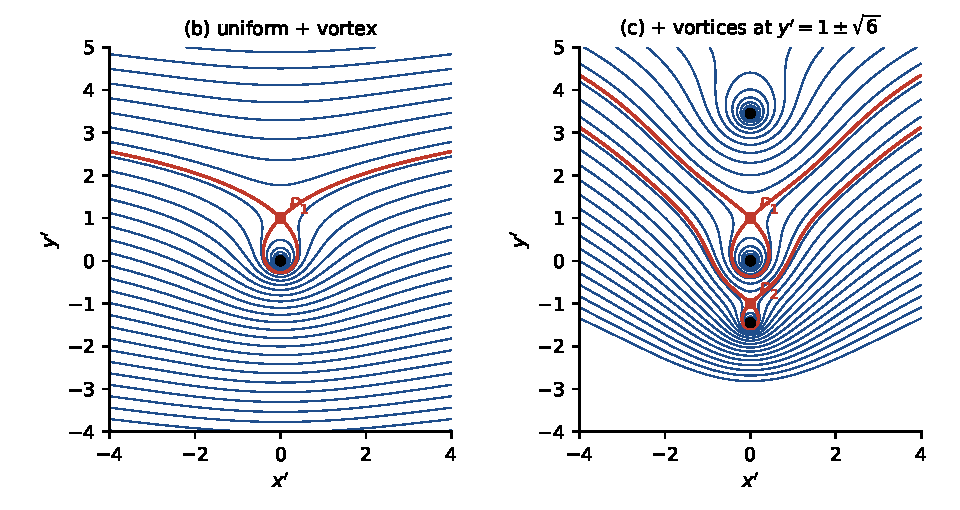
\includegraphics[width=0.95\textwidth]{t25_p3.pdf}
\end{center}
Red: streamlines through the stagnation points (the dividing streamlines). Black dots: vortex centres.

%==================================================================
\section*{Problem 4 \normalsize(4.0 p.)}

\begin{strategy}
Keywords: \kw{long plates}, \kw{steady}, \kw{$u=w=0$} $\Rightarrow$ everything depends on $y$ only.
\kw{porous}, \kw{$v_0$ at the plates} $\Rightarrow$ continuity gives $v=v_0$ everywhere.
\kw{Boussinesq} $\Rightarrow$ $\nabla\!\cdot\bu=0$, $\rho_0$ everywhere except in the gravity term, where $\rho=\rho_0-\alpha(T-T_0)$.
Temperature: the energy equation with \emph{advection} ($v_0T'$) balancing conduction. No dissipation, since $v$ is uniform.
Pressure: $y$-momentum, which reduces to hydrostatics with the variable density $\rho(T(y))$.
\end{strategy}

\textbf{Notation.} The plates are at $y=0$ (temperature $T_0$, pressure $p_0$) and $y=b$ (temperature $T_0-\Delta T$). We write $b$ for the gap, which the statement does not name.

\subsection*{(a) Velocity and temperature}
\textbf{Continuity (Boussinesq: incompressible).} $\pd_xu+\pd_yv+\pd_zw=\frac{dv}{dy}=0\ \Rightarrow\ v=$ const $=v_0$ (value at the plates).
\[
\boxed{\bu=(0,\ v_0,\ 0)}
\]

\textbf{Energy equation.} Steady, with $T=T(y)$: $\rho_0c_p\,v\,\frac{dT}{dy}=\lambda\frac{d^2T}{dy^2}+\Phi$. The viscous dissipation $\Phi=2\mu(\pd_yv)^2=0$ because $v$ is uniform. With $\kappa=\lambda/(\rho_0c_p)$:
\[
v_0T'=\kappa T''\quad\Longrightarrow\quad T''-\frac{v_0}{\kappa}T'=0 .
\]
Characteristic roots: $\lambda=0$ and $\lambda=v_0/\kappa$, so $T=C_1+C_2e^{v_0y/\kappa}$.

BCs $T(0)=T_0$, $T(b)=T_0-\Delta T$ give $C_1+C_2=T_0$ and $C_2\left(e^{v_0b/\kappa}-1\right)=-\Delta T$:
\[
\boxed{T(y)=T_0-\Delta T\,\frac{e^{v_0y/\kappa}-1}{e^{v_0b/\kappa}-1}}
\]
\textbf{Interpretation.} The upward flow carries the heat of the lower plate upwards, so most of the gap stays near $T_0$. The temperature drops in a layer of thickness $\sim\kappa/v_0$ next to the upper plate. The ratio $Pe=v_0b/\kappa$ (Péclet number) measures advection vs.\ conduction.

\subsection*{(b) Pressure}
\textbf{$x$- and $z$-momentum:} all terms vanish except $-\pd_xp=0$, $-\pd_zp=0$, so $p=p(y)$.

\textbf{$y$-momentum:} $\rho_0\,v\,\pd_yv=-\pd_yp-\rho g+\mu\pd_y^2v$. The inertial and viscous terms vanish ($v$ constant), leaving hydrostatics with the temperature-dependent density:
\[
\frac{dp}{dy}=-\rho g=-g\left[\rho_0-\alpha\left(T-T_0\right)\right]=-\rho_0g-g\alpha\Delta T\,\frac{e^{v_0y/\kappa}-1}{e^{v_0b/\kappa}-1}.
\]
Integrate from $0$ to $y$ with $p(0)=p_0$, using $\int_0^y\left(e^{v_0s/\kappa}-1\right)ds=\frac{\kappa}{v_0}\left(e^{v_0y/\kappa}-1\right)-y$:
\[
\boxed{p(y)=p_0-\rho_0gy-\frac{g\alpha\Delta T}{e^{v_0b/\kappa}-1}\left[\frac{\kappa}{v_0}\left(e^{v_0y/\kappa}-1\right)-y\right]}
\]
The first two terms are the hydrostatic pressure of the reference density. The bracket is $\ge0$: the fluid is colder ($T\le T_0$), hence denser, than the reference, so the pressure decreases faster with height.

\subsection*{(c) Limit $v_0\to0$}
Let $s=v_0/\kappa\to0$ and expand $e^{sy}-1\simeq sy+\frac{s^2y^2}{2}$.

\emph{Temperature:} $\dfrac{e^{sy}-1}{e^{sb}-1}\to\dfrac{y}{b}$, so
\[
\boxed{T(y)=T_0-\Delta T\,\frac{y}{b}}
\]
the linear profile of pure conduction. Equivalently, set $v_0=0$ directly: $T''=0$.

\emph{Pressure:} $\dfrac{1}{e^{sb}-1}\left[\dfrac{e^{sy}-1}{s}-y\right]\simeq\dfrac{1}{sb}\cdot\dfrac{sy^2}{2}=\dfrac{y^2}{2b}$, so
\[
\boxed{p(y)=p_0-\rho_0gy-\frac{\alpha g\Delta T}{2b}\,y^2}
\]
This also follows from $dp/dy=-g[\rho_0+\alpha\Delta T\,y/b]$ with the linear temperature.

\why{Remark: the fluid is heated from below, so the denser (colder) fluid sits on top. This rest/through-flow state is the \emph{base state} of Rayleigh--Bénard convection. It is the actual solution only while the temperature difference is small enough that the configuration remains stable; the problem assumes this by imposing $u=w=0$.}

\end{document}
